\chapter{Graphs and plots}
\label{chap-graphs}

\section{Gnuplot graphs}
\label{gnuplot-graphs}

A separate program, \app{gnuplot}, is called to generate graphs.
Gnuplot is a very full-featured graphing program with myriad options.
It is available from \href{http://www.gnuplot.info/}{www.gnuplot.info}
(but note that a suitable copy of gnuplot is bundled with the packaged
versions of \app{gretl} for MS Windows and Mac OS X).  \app{gretl}
gives you direct access, via a graphical interface, to a subset of
gnuplot's options and it tries to choose sensible values for you; it
also allows you to take complete control over graph details if you
wish.

With a graph displayed, you can click on the graph window for a pop-up
menu with the following options.

\begin{itemize}
\item \textsf{Save as PNG}: Save the graph in Portable Network
  Graphics format.
\item \textsf{Save as postscript}: Save in encapsulated postscript
  (EPS) format.
\item \textsf{Save as Windows metafile}: Save in Enhanced Metafile
  (EMF) format.
\item \textsf{Save to session as icon}: The graph will appear in
  iconic form when you select ``Icon view'' from the View menu.
\item \textsf{Zoom}: Lets you select an area within the graph for
  closer inspection (not available for all graphs).
\item \textsf{Print}: (Gnome desktop or MS Windows only) lets you
  print the graph directly.
\item \textsf{Copy to clipboard}: MS Windows only, lets you paste the
  graph into Windows applications such as MS Word.
\item \textsf{Edit}: Opens a controller for the plot which lets you
  adjust many aspects of its appearance.
\item \textsf{Close}: Closes the graph window.
\end{itemize}


\subsection{Displaying data labels}
\label{plot-labels}

In the case of a simple X-Y scatterplot (with or without a line of
best fit displayed), some further options are available if the dataset
includes ``case markers'' (that is, labels identifying each
observation).\footnote{For an example of such a dataset, see the
  Ramanathan file \verb+data4-10+: this contains data on private
  school enrollment for the 50 states of the USA plus Washington, DC;
  the case markers are the two-letter codes for the states.} With a
scatter plot displayed, when you move the mouse pointer over a data
point its label is shown on the graph.  By default these labels are
transient: they do not appear in the printed or copied version of the
graph.  They can be removed by selecting ``Clear data labels'' from
the graph pop-up menu. If you want the labels to be affixed
permanently (so they will show up when the graph is printed or
copied), you have two options.
    
\begin{itemize}
\item To affix the labels currently shown on the graph, select
  ``Freeze data labels'' from the graph pop-up menu.
\item To affix labels for all points in the graph, select ``Edit''
  from the graph pop-up and check the box titled ``Show all data
  labels''.  This option is available only if there are less than 55
  data points, and it is unlikely to produce good results if the
  points are tightly clustered since the labels will tend to overlap.
\end{itemize}

To remove labels that have been affixed in either of these ways,
select ``Edit'' from the graph pop-up and uncheck ``Show all data
labels''.
    

\subsection{Advanced options}
\label{plot-advanced}

If you know something about \app{gnuplot} and wish to get finer
control over the appearance of a graph than is available via the
graphical controller (``Edit'' option), here's what to do.  In the
graph display window, right-click and choose ``Save to session as
icon''.  Then open the icon view window --- either via the menu item
View/Icon view, or by clicking the ``session icon view'' button on the
main-window toolbar.  You should see an icon representing your graph.
Right-click on that and select ``Edit plot commands'' from the pop-up
menu.  This opens an editing window with the actual gnuplot commands
displayed. You can edit these commands and either save them for future
processing or send them to \app{gnuplot} directly, using the Execute
(cogwheel) button on the toolbar in the plot commands editing window.

To find out more about \app{gnuplot} visit
\href{http://www.gnuplot.info/}{www.gnuplot.info}. This site has
documentation for the current version of the program in various
formats.  

See also the entry for \cmd{gnuplot} in the \GCR\ --- and the
\cmd{graph} and \cmd{plot} commands for ``quick and dirty'' ASCII
graphs.

\begin{figure}[htbp]
  \begin{center}
    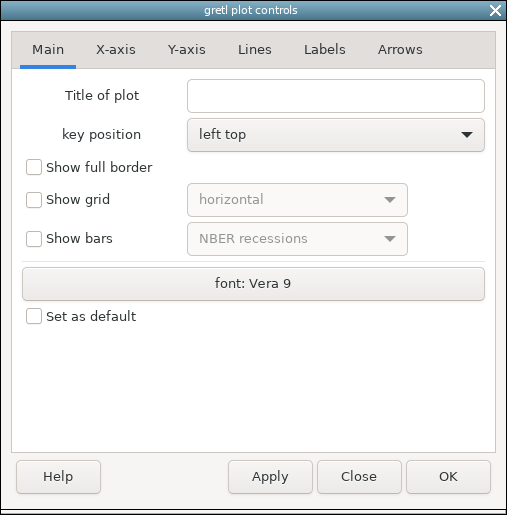
\includegraphics[scale=0.5]{figures/plot_control}
  \end{center}
  \caption{gretl's gnuplot controller}
  \label{fig-plot}
\end{figure}


\section{Boxplots}
\label{sect-boxplots}

These plots (after Tukey and Chambers) display the distribution
of a variable. The central box encloses the middle 50 percent of the
data, i.e.\ it is bounded by the first and third quartiles.  The
``whiskers'' extend to the minimum and maximum values.  A line is
drawn across the box at the median and a ``\texttt{+}'' sign
identifies the mean.

In the case of boxplots with confidence intervals, dotted lines show
the limits of an approximate 90 percent confidence interval for the
median.  This is obtained by the bootstrap method, which can take a
while if the data series is very long.

After each variable specified in the boxplot command, a parenthesized
boolean expression may be added, to limit the sample for the variable
in question.  A space must be inserted between the variable name or
number and the expression.  Suppose you have salary figures for men
and women, and you have a dummy variable \verb+GENDER+ with value 1
for men and 0 for women.  In that case you could draw comparative
boxplots with the following line in the boxplots dialog:

\begin{code}
salary (GENDER=1) salary (GENDER=0)
\end{code}

%%% Local Variables: 
%%% mode: latex
%%% TeX-master: "gretl-guide"
%%% End: 

